The aim of this proposal is to (1) identify a set of principles for the analysis (formal, static,
  and dynamic) of communication protocols and
  their implementations in embedded systems; (2) implement these theoretical principles in tools usable by
  engineers developing such systems; and (3) use these tools in two real applications.
  In the first case study, we will formally, statically, and dynamically analyze networks
  of wireless sensor/actuator nodes deployed in the Southwest Experimental Garden
  Array (SEGA)~\cite{YamEtAl10,FliEtAl12}, a distributed facility for
  examining climatic, genetic, and environmental factors in plant ecology.
  The second case study will use the tools to formally verify and dynamically test the distributed coordination code of multiple autonomous ground and aerial robots in a lab setting.


\begin{figure}[!t]
  \centering
  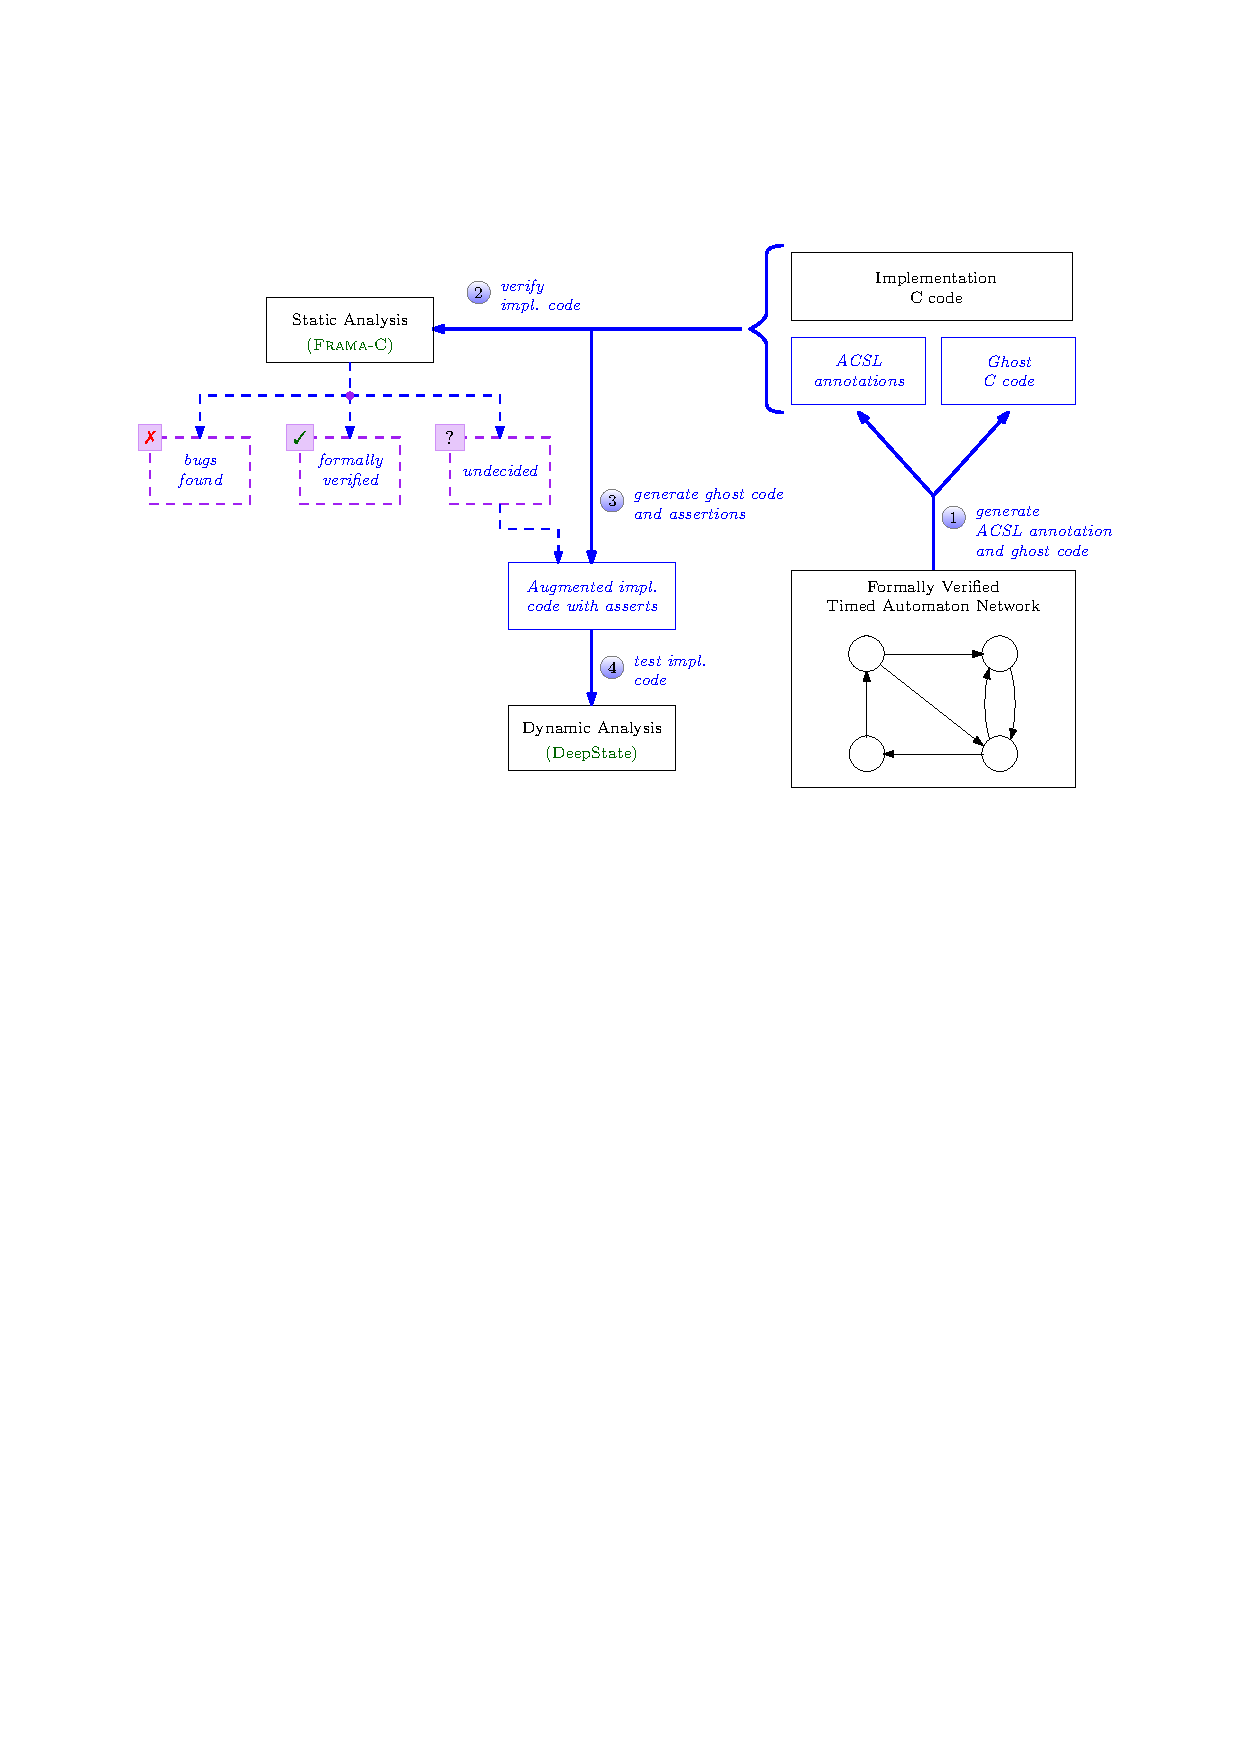
\includegraphics[width=.8\textwidth]{overview}
  \caption{Overview of the proposed research.}
  \label{fig:overview}
\end{figure}

Figure~\ref{fig:overview} shows the overall concept.  The core
open research problems addressed are represented by two sets of
arrows.  First, an engineering design, modeled as a network of timed
automata (TA), is formally verified with respect to a set of temporal logic specifications.
The timed automaton modeling paradigm together with temporal logics
for system requirements are rich enough for expressing many practical
engineering system designs, including but not limited to communication
protocols and supervisory controls (including those relevant to sensor
networks and IoT systems).  Existing C code that is supposed to
implement the design, and hence satisfy the design specifications, is provided and needs to be verified.
Our goal is to certify whether the C code truly implements the complete TA-based design and, if not, find any bugs in the code:
\begin{enumerate}[labelsep=3pt,leftmargin=12pt]
\item First, from the TA, \acsl annotations\footnote{\acsl is the
    specification language of \framac{}.} and possibly ghost C code
  (code that does not contribute to runtime semantics, but assists in
  proof construction) are automatically generated to augment the
  implementation code. The annotations together with ghost code
  describe the semantics of the TA: if
  the annotated specification can be verified, then the TA design is implemented correctly.
\item The implementation code with the \acsl annotations and ghost code
  is verified by a static analysis tool, in our case \framac.
  There are three possible outcomes:
  {\bf verified:} the implementation can be formally verified, which means that it correctly implements the TA design and therefore meets the design specifications;
  {\bf bugs found:} bugs are found in the implementation, showing that
    it can violate the specification, and the bugs must be fixed; and
  {\bf undecided:} the static analysis tool is unable to prove or disprove correctness of the implementation,
  in which case, we continue with the next step.
\item In the event of an undecided outcome from the static analysis
  step, we attempt to refute correctness (or increase our confidence
  in it) via dynamic analysis---automated test generation.
  Ghost code, runtime assertions, and test-harness are \emph{automatically generated} from the
  annotated code.
\item The augmented implementation code is then analyzed using the
  \deepstate~\cite{DeepState} framework.  Generated test cases may
  prove the system faulty, or they may leave us more confident
  the system is correct.
\end{enumerate}

\paragraph{Principles:} Assuming that a communication protocol is described
as (probabilistic) timed automata~\cite{AD1994:TCS},
which satisfy temporal logic
formulas~\cite{BLM2017:LNCS}, and implemented as a set of
imperative programs, we ask:
\begin{itemize}[labelsep=3pt,leftmargin=12pt]
\item Given the timed automata and a set of programs supposed to
  implement them, how can we annotate the programs to be able to check
  that they correctly implement the protocol, or to find bugs?
\item Given a set of annotated programs, how can we automatically
  generate a test harness for the system?
\end{itemize}
% REMOVED MENTIONS OF THE TOY LANGUAGE
%For the first problem, we will consider a toy imperative language with the
%usual control structures, unbounded integers, addresses, and
%non-recursive procedures.

Note that these problems differ considerably from the more studied,
but more limited, synthesis problem.  We are not assuming that
system development will involve first producing a formal model, then
using that model to automatically generate an implementation; rather,
we consider the typical real-world scenario, where modeling is a
separate activity, either undertaken after implementation due to
concerns about reliability, or an activity during design that only
indirectly informs the implementation.  That is, the more studied
problem is producing a runtime semantics for a model; we address the
problem of reconciling a model semantics and a runtime semantics,
without unrealistic burden on engineers.


\paragraph{Tools:} We will focus on C code, using \framac~\cite{KKP2015:FAC} and \deepstate~\cite{DeepState}
for the analysis of code, and
\uppaal~\footnote{\url{http://www.uppaal.org}} and
\prism~\cite{KNP2011:CAV}) for the analysis of protocols.  The primary open research questions here are numerous, and include:
% (1) how to handle C constructs that are not part of the toy language;
(1) how to extend existing specification languages to support timing and uncertainty;
(2) how to assign the same meaning to a specification construct in
  the static \framac context and the dynamic \deepstate context;
(3) how to handle intra-program parallelism;
(4) how to effectively translate a failed proof effort in \framac
  into a representation of a testing problem (to find counterexamples
  refuting that proof could be possible) in a dynamic setting; and
(5) how to ensure that the methods are sufficiently automatic
  and behave in ways engineers (not modeling, static, or dynamic
  analysis experts) will expect.

Our focus will be on \emph{practical} solutions, guided by the
embedded domain experts, rather than on purely theoretical approaches
that do not scale to real systems. Practical solutions here require
fundamental contributions to system and specification design and
semantics and static and dynamic analysis methods.